\documentclass[letterpaper,10pt,conference]{ieeeconf}
\IEEEoverridecommandlockouts
\overrideIEEEmargins
\let\proof\relax
\let\endproof\relax
\usepackage{amsmath,amssymb,amsthm,mathtools}
\usepackage{graphicx,booktabs,array,cite}
\usepackage[hidelinks]{hyperref}
\usepackage{tikz}
\usetikzlibrary{patterns,calc}
\usepackage[caption=false,font=footnotesize,farskip=0pt,captionskip=3pt]{subfig}
\usepackage[hidelinks]{hyperref}
\usepackage{microtype}
\usepackage{placeins}
\graphicspath{{figures/}}
\setcounter{topnumber}{4}\setcounter{totalnumber}{6}\setcounter{dbltopnumber}{4}
\renewcommand{\topfraction}{0.95}\renewcommand{\dbltopfraction}{0.95}\renewcommand{\textfraction}{0.05}\renewcommand{\floatpagefraction}{0.5}\renewcommand{\dblfloatpagefraction}{0.5}
% space between two figures and between a figure and the text (the class sets 0.85 and 1.55 baselines)
\setlength{\floatsep}{6pt plus 2pt minus 2pt}\setlength{\textfloatsep}{8pt plus 2pt minus 2pt}
\setlength{\dblfloatsep}{6pt plus 2pt minus 2pt}\setlength{\dbltextfloatsep}{8pt plus 2pt minus 2pt}

% Theorem-like environments and notation of the paper.

% ---------- theorem-like environments (one shared counter) ----------
\newtheorem{definition}{Definition}
\newtheorem{lemma}[definition]{Lemma}
\newtheorem{theorem}[definition]{Theorem}
\newtheorem{proposition}[definition]{Proposition}
\newtheorem{assumption}[definition]{Assumption}
\theoremstyle{remark}
\newtheorem{remark}[definition]{Remark}

% ---------- notation ----------
\newcommand{\R}{\mathbb{R}}
\newcommand{\Sph}{\mathbb{S}^{2}}
\newcommand{\Dres}{\mathsf{D}}
\newcommand{\Drel}{\Dres^{\mathrm{rel}}}
\newcommand{\Xop}{\mathcal{X}_{\mathrm{op}}}
\newcommand{\Xrf}{\mathcal{X}_{\mathrm{RF}}}
\newcommand{\Cho}{\mathcal{C}_{\mathrm{HO}}}
\newcommand{\Viab}{\operatorname{Viab}}
\newcommand{\pos}[1]{{(#1)}_{+}}
\newcommand{\negp}[1]{{(#1)}_{-}}
\newcommand{\tr}{^{\!\top}}
\newcommand{\plan}{\pi^{\sharp}}
\newcommand{\ua}{\underline{\alpha}}
\newcommand{\oa}{\overline{\alpha}}


\begin{document}

\title{Explicit Viability Bounds for Safety Filters with Configuration-Dependent Braking Authority}

\author{%
Hadi Hajieghrary$^{1}$ and Paul Schmitt$^{2}$%
\thanks{$^{1}$Hadi Hajieghrary (e-mail: \texttt{hadi.hajieghrary@gatech.edu}).}%
\thanks{$^{2}$Paul Schmitt (e-mail: \texttt{pauls@massrobotics.org},\hfil\break \texttt{paul.schmitt@reynolds-moore.com}).}%
\thanks{The authors prepared this manuscript and present it solely in their individual capacities.}%
}

\maketitle

\begin{abstract}
%A cable-suspended payload may approach a wall while every cable pulls it toward the wall; the quadrotors must first swing behind the payload before they can brake. A high-order control barrier function (HOCBF) filter that admits an input now can lose feasibility during this swing, and we give a condition under which it must, with a two-quadrotor example. We then derive an explicit certificate. A thrust-reserved swing-and-brake maneuver that carries the payload weight has an exactly computable stopping distance, yielding an authority barrier and two altitude barriers; their certified set is control-invariant for the continuous-time taut-cable model, provided closed-loop solutions exist and the braking maneuver remains feasible for the resulting filter. An optimistic stopping distance bounds the viability kernel from outside. Both distances use the support function of the zonotope of tension forces, which depends on the cable directions. In the exact model with a $1\,\mathrm{ms}$ hold, one of 100 trials starting at the boundary of the certified set reaches the wall by $2\,\mu\mathrm m$. Simulations expose substantial conservatism when swinging is required, and wall contacts under a slower sampled filter and a slack-cable model.

A team of quadrotors carrying a cable-suspended payload may need to reposition before it can brake near an obstacle.  If all cables pull toward a wall, the team cannot slow the payload until the cable directions change.  This delay can cause a safety filter to accept a control input now and become infeasible later.  We derive a condition for this failure in a wall-distance high-order control barrier function (HOCBF) filter.  We address the delay using the analytically computable stopping distance of a feasible swing-and-brake maneuver.  The maneuver reserves thrust for repositioning while supporting the payload’s weight.  Under the stated assumptions, the resulting certificate defines a controlled-invariant set for the continuous-time taut-cable model.  The proposed safety filter remains feasible throughout this set.  A complementary optimistic model identifies states from which no admissible controller can prevent wall contact.  Simulations compare the proposed filter with HOCBF filters. Of 100 trials started at its boundary with a hold of 1 ms, only one reaches the wall, by 2 micrometers, and none does with a hold of 0.5 ms. The certificate is conservative where a swing is required, and with a 5 ms hold and slack cables many trials make contact; we report this as the clearest limitation.

\end{abstract}

\section{Introduction}
A quadrotor can pull a cable-suspended payload but cannot push it. If all quadrotors are between a moving payload and a wall, changing the tensions cannot brake the payload; a quadrotor first has to swing to its far side (Fig.~\ref{fig:scene}). This delay is hidden by a high-order control barrier function (HOCBF) that tests only the currently achievable acceleration. We quantify the delay and construct a safety certificate from the maximum wallward excursion of a feasible braking maneuver.

Input-constrained HOCBFs~\cite{xiao2022high,breeden2021high}, feasibility constraints~\cite{xiao2022sufficient}, and backup, constructive, and predictive CBFs~\cite{chen2021backup,vanwijk2025,squires2018constructive,breeden2022predictive} address feasibility through different safe sets; backup CBFs keep racing drones inside a geofence~\cite{singletary2022onboard}, and the braking-distance barrier of adaptive cruise control~\cite{ames2014control} is the special case of a constant authority. Cable-robot wrench calculations describe forces available at a fixed geometry, as intervals or zonotopes~\cite{gouttefarde2011interval,bouchard2010ability,erskine2019wrench}; aerial transport models describe how that geometry moves~\cite{sreenath2013dynamics,lee2018geometric}, and CBFs have been used to plan cable transport~\cite{pallar2025optimal}. Concurrently,~\cite{shi2026escape} certifies a quadrotor that must reorient its thrust before it can brake, with a body-rate model of first order; here the authority follows from the cable geometry, the swing is of second order, and the same calculation gives an outer bound. Closed-form backup control is also studied in~\cite{vanwijk2025}; our closed form concerns the future wall excursion for this particular authority model.

\begin{figure}[t]
\centering

\resizebox{\columnwidth}{!}{%
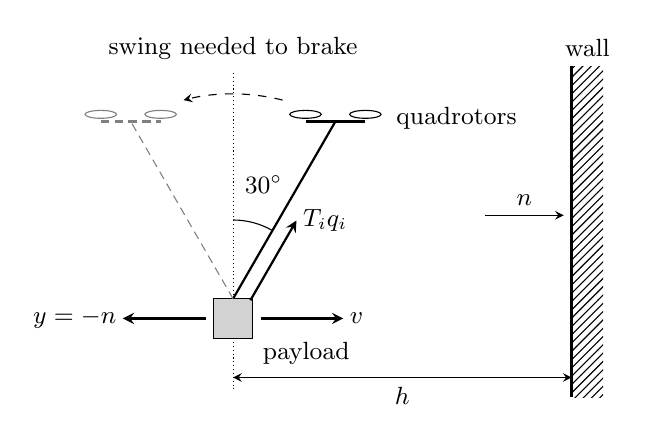
\begin{tikzpicture}[x=1cm,y=1cm,>=stealth,font=\small]

% wall
\fill[pattern=north east lines] (7.6,0.0) rectangle (8.0,4.20);

\draw[very thick] (7.6,0.0) -- (7.6,4.20);

\node[anchor=south] at (7.8,4.20) {wall};

\draw[->] (6.5,2.31) -- (7.5,2.31)
    node[midway,anchor=south] {$n$};

% payload
\filldraw[fill=gray!35,draw=black] (3.05,0.75) rectangle (3.55,1.25);

\node[anchor=north west,inner sep=2pt] at (3.6,0.78) {payload};

\coordinate (A) at (3.3,1.25);

% vertical through the payload and the angle of the cables
\draw[densely dotted] (A) -- ++(0,2.90);

\draw (A) ++(90:1.0) arc[start angle=90,end angle=60,radius=1.0];

\node at ($(A)+(75:1.5)$) {$30^\circ$};

% cables and quadrotors, leaning toward the wall
\draw[thick] (A) -- ++(60:2.60) coordinate (Q);

\draw[very thick] ($(Q)+(-0.38,0)$) -- ($(Q)+(0.38,0)$);

\draw ($(Q)+(-0.38,0.09)$) ellipse [x radius=0.2,y radius=0.05];

\draw ($(Q)+(0.38,0.09)$) ellipse [x radius=0.2,y radius=0.05];

\node[anchor=west] at ($(Q)+(0.65,0.04)$) {quadrotors};

\draw[->,thick] ($(A)+(0.22,-0.02)$) -- ++(60:1.17)
    node[anchor=west,inner sep=2pt] {$T_iq_i$};

% cables and quadrotors after the swing
\draw[densely dashed,gray] (A) -- ++(120:2.60) coordinate (G);

\draw[densely dashed,gray,very thick] ($(G)+(-0.38,0)$) -- ($(G)+(0.38,0)$);

\draw[gray] ($(G)+(-0.38,0.09)$) ellipse [x radius=0.2,y radius=0.05];

\draw[gray] ($(G)+(0.38,0.09)$) ellipse [x radius=0.2,y radius=0.05];

\draw[dashed,->] ($(A)+(76:2.60)$)
    arc[start angle=76,end angle=104,radius=2.60];

\node[anchor=south] at ($(A)+(90:2.92)$) {swing needed to brake};

% velocity and braking direction
\draw[->,thick] (3.65,1.0) -- (4.7,1.0)
    node[anchor=west,inner sep=2pt] {$v$};

\draw[->,thick] (2.95,1.0) -- (1.9,1.0)
    node[anchor=east,inner sep=2pt] {$y=-n$};

% distance to the wall
\draw[densely dotted] (3.3,0.75) -- (3.3,0.1);

\draw[<->] (3.3,0.25) -- (7.6,0.25)
    node[midway,anchor=north] {$h$};

\end{tikzpicture}%
}

\caption{Two quadrotors carry a payload toward a wall. With both cables leaning toward the wall, positive tensions cannot brake it; a cable must first swing to the far side (dashed).}

\label{fig:scene}

\end{figure}

We let each quadrotor reserve part of its thrust for the cable tension and part for swinging the cable; the braking authority that this guarantees is the support function of the zonotope of tension forces and depends on the cable directions alone (Sec.~\ref{sec:theory}). When every cable swings to its limit, the payload covers at most the stopping distance $\Dres$ toward the wall, which is computed exactly (Sec.~\ref{sec:barrier}). The authority barrier is $H:=h-\Dres$: the states with $H\ge0$ and admissible swing states form a controlled-invariant set, in which the braking maneuver satisfies every constraint of the filter of Sec.~\ref{sec:filter}; two further barriers bound the altitude of the payload during the maneuver. With upper bounds on the authority and on the swing acceleration, the same calculation gives an optimistic stopping distance $\Drel$, below which no state is viable (Theorem~\ref{thm:sandwich}). Both bounds hold for every system whose braking authority is bounded by nondecreasing functions of coordinates that the inputs drive only through their second derivative (Sec.~\ref{sec:class}); the cable system is one instance.

The contributions are: (i) a condition under which an initially feasible HOCBF filter must lose feasibility before a cable reaches the braking half-space (Theorem~\ref{thm:negative}); (ii) an explicit stopping distance for the input-constrained taut-cable model, the authority and altitude barriers built from it, and the certified set on which the barrier filter is always feasible (Theorem~\ref{thm:sandwich}(i), Proposition~\ref{prop:instance}); (iii) an explicit outer bound on the viability kernel (Theorem~\ref{thm:sandwich}(ii)); and (iv) simulations that test the certificate on its own model and measure its conservatism and the failure of a direct sampled implementation. In simulation, the HOCBF filter lost feasibility in all 690 trials; on the exact model with a $1\,\mathrm{ms}$ hold the authority filter reached the wall in one of 100 trials started at the boundary of its certified set, by $2\,\mu\mathrm m$; on the full-order model with a $5\,\mathrm{ms}$ hold and the wall barrier alone it reached the wall in 59 of 100. The sampled results concern the implementation and give no safety guarantee.



\section{Problem Formulation}\label{sec:problem}

Quadrotor $i\in\{1,\dots,N\}$ has position $p_i\in\R^3$, mass $m_i$, and thrust vector $u_i:=f_iR_ie_3$, where $f_i\ge0$ is the thrust magnitude, $R_i\in SO(3)$ the attitude, and $e_3$ the vertical unit vector; an attitude controller produces the commanded thrust vectors (Remark~\ref{rem:inner}). Each thrust vector lies in the ball $\mathcal{F}_i:=\{u\in\R^3:\ \|u\|\le f_{\max,i}\}$; a tilt limit can be added to $\mathcal{F}_i$ as long as Assumption~\ref{ass:split} is checked with it.

The payload is a point mass $m_L$ at $x_L\in\R^3$, attached to quadrotor $i$ by a massless, inextensible cable of length $l_i$ with unit direction $q_i\in\Sph$ from the payload to the quadrotor, $p_i=x_L+l_iq_i$. The cable exerts the force $T_iq_i$ on the payload and $-T_iq_i$ on the quadrotor, with $T_i\ge0$ because a cable cannot push. With disturbance forces $d_L$, $d_i$ and the gravitational acceleration $g$,
\begin{align}
m_L\ddot x_L &= \textstyle\sum_{i} T_i q_i - m_L g e_3 + d_L, \label{eq:load}\\
m_i\ddot p_i &= u_i - m_i g e_3 - T_i q_i + d_i. \label{eq:veh}
\end{align}
The state is $x:=(x_L,\dot x_L,q,\dot q)$ with $q:=(q_1,\dots,q_N)$. In this work, we assume that every cable is taut, with a tension of at least $T_{\min}>0$; the filter of Sec.~\ref{sec:filter} enforces this bound, and the simulations model slack cables.

We decompose each thrust vector along the cable and perpendicular to it, $u_i=s_iq_i+u_i^{\perp}$ with $s_i:=q_i\tr u_i$, $u_i^\perp:=P_iu_i$, $P_i:=I-q_iq_i\tr$, and we use the \emph{specific force} of the payload, $a:=\ddot x_L+ge_3$, which an accelerometer on the payload measures. Differentiating $\|p_i-x_L\|=l_i$ twice and substituting \eqref{eq:load}--\eqref{eq:veh} gives the following.

\begin{lemma}[Structure]\label{lem:structure}
Along any solution of \eqref{eq:load}--\eqref{eq:veh} with taut cables:
(a) $T_i = s_i - m_i\,q_i\tr a + m_i l_i\|\dot q_i\|^2 + q_i\tr d_i$, so the tension depends on the inputs only through the parallel components $s=(s_1,\dots,s_N)$;
(b) $\ddot q_i = \tfrac{1}{m_il_i}u_i^\perp - \tfrac{1}{l_i}P_i a - \|\dot q_i\|^2 q_i + \tfrac{1}{m_il_i}P_id_i$, so the cable direction depends on the inputs only through $u_i^\perp$ and $a$;
(c) $M_a(q)\,a=\sum_i s_iq_i+\sum_i m_il_i\|\dot q_i\|^2q_i+\sum_i (q_i\tr d_i)q_i+d_L$ with $M_a(q):=m_LI+\sum_i m_iq_iq_i\tr\succeq m_LI$, so $a$ is affine in $s$;
(d) for a given $a$, (a) and (b) involve only the quantities of quadrotor $i$.
\end{lemma}
\begin{proof}[Proof scheme]
Differentiate $p_i=x_L+l_iq_i$ twice. Since $q_i^\top\dot q_i=0$ and $q_i^\top\ddot q_i=-\|\dot q_i\|^2$, projecting the vehicle equation along $q_i$ isolates $T_i$ and gives (a). Projecting perpendicular to $q_i$ removes the tension and gives (b). Substituting (a) into the payload equation gives (c). For any nonzero $r$, $r^\top M_a r=m_L\|r\|^2+\sum_i m_i(q_i^\top r)^2>0$, so $a$ is uniquely determined by the parallel thrusts. The remaining local dependences in (d) follow directly.
\end{proof}

In words, the parallel component sets the tension, the perpendicular component swings the cable, the two share the limit $\|s_iq_i+u_i^\perp\|\le f_{\max,i}$, and the quadrotors interact only through the payload's specific force. For fixed $(q,\dot q)$, (a) and (c) define an affine bijection between $s$ and $T=(T_1,\dots,T_N)$, so we use the tensions as decision variables: given $T$, $a=\frac{1}{m_L}(\sum_jT_jq_j+d_L)$, and (a) returns $s_i(T)$.

\subsection{Wall constraint, safe set, and admissible inputs}

We consider a wall with horizontal unit normal $n$ pointing into it, with the constraint
\begin{equation}
h(x_L):=d_0-n\tr x_L\ge 0,
\label{eq:h}
\end{equation}
where $h$ is the distance from the payload to the wall. We write $v:=n\tr\dot x_L$ for the approach speed, $y:=-n$ for the braking direction, and $b:=y\tr\ddot x_L$ for the braking deceleration, so that $\dot h=-v$ and $\dot v=-b$, and we describe each cable direction by $z_i:=q_i\tr y$ and $w_i:=q_i\tr r$, $r:=e_3\times y$. A cable with $z_i>0$ leans away from the wall and pulls the payload away from it; one with $z_i<0$ pulls it toward the wall.

We impose the operational constraints
\begin{equation}
\Xop:=\{x:\ |z_i|\le\bar z,\ (w_i,\dot w_i)\in\mathcal V(\nu_w,\bar w),\ \|\dot q_i\|\le\bar\omega\ \forall i\},
\label{eq:Xop}
\end{equation}
with $\bar z^2+\bar w^2\le\sin^2\theta_q$, $\theta_q<\pi/2$, which keep every cable within $\theta_q$ of the vertical, reserve stopping room for the transverse swing, and bound its swing rate; $\mathcal V$ is defined in \eqref{eq:box} below. The safe set is $\mathcal{C}:=\{x:\ h\ge 0\}\cap\Xop$. The inputs must respect the thrust limits, the tension bound, and a bound $a_{\max}$ on the payload's specific force:
\begin{equation}
\begin{split}
\mathcal{U}(x):=\{u:\ &u_i\in\mathcal{F}_i,\ T_i(x,u)\ge T_{\min}\ \forall i,\\ &\textstyle\|\sum_iT_i(x,u)q_i\|\le m_La_{\max}\}.
\end{split}
\label{eq:U}
\end{equation}
The last constraint is a design limit on the payload's acceleration; the bound that follows from the thrust limits alone, $\frac{1}{m_L}\sum_j(f_{\max,j}+m_jl_j\bar\omega^2)$, is too large for Assumption~\ref{ass:split} to hold with realistic constants.

Tensions affect $\ddot h$ directly, whereas a transverse input first changes $\ddot q_i$ and thereby later changes the feasible braking force.

A state is \emph{viable} if some input signal with values in $\mathcal{U}(x)$ keeps the trajectory in $\mathcal{C}$ forever; the set of viable states is the \emph{viability kernel} $\Viab(\mathcal{C})$ \cite{aubin1991viability}, outside of which no controller can keep the system safe. A set is \emph{controlled invariant} if some admissible input signal keeps every trajectory that starts in it inside it; every controlled-invariant subset of $\mathcal{C}$ lies in $\Viab(\mathcal{C})$, which has no closed form. The problem is: (a) find a controlled-invariant set $\mathcal{S}\subseteq\mathcal{C}$ whose membership can be tested online; (b) find an explicit set that contains $\Viab(\mathcal{C})$; and (c) derive a safety filter that is feasible at every state of $\mathcal{S}$.



\section{Loss of Feasibility of High-Order CBF Filters}\label{sec:negative}

For a unit vector $y$, the \emph{exact directional authority} at $x$,
\begin{equation}
\alpha^{\mathrm{ex}}_y(x):=\max\{\,y\tr\ddot x_L(x,u):\ u\in\mathcal{U}(x)\,\},
\label{eq:exact}
\end{equation}
is the largest acceleration that admissible inputs can give the payload along $y$; the maximum exists because $\ddot x_L$ is affine in $u$ and $\mathcal{U}(x)$ is compact and convex ($-\infty$ if empty). Since it is attained, for any function $\beta$ of the state,
\begin{equation}
\{u\in\mathcal{U}(x):\ b(x,u)\ge\beta(x)\}\ne\emptyset\iff\alpha^{\mathrm{ex}}_y(x)\ge\beta(x).
\label{eq:iff}
\end{equation}

Since $h$ has relative degree two with respect to the tensions, HOCBFs \cite{xiao2019control,nguyen2016exponential} apply the barrier condition twice. Let $\alpha_1$ be a continuously differentiable class-$\mathcal{K}$ function, $\alpha_2$ an extended class-$\mathcal{K}$ function, and $\psi_1:=\dot h+\alpha_1(h)=-v+\alpha_1(h)$. With $\dot v=-b$, the HOCBF condition $\dot\psi_1\ge-\alpha_2(\psi_1)$ reads
\begin{equation}
b\ \ge\ \beta(x):=\alpha_1'(h)\,v-\alpha_2(\psi_1).
\label{eq:hocbf}
\end{equation}
The HOCBF filter minimizes the change to the nominal command over $K_{\mathrm{HO}}(x):=\{u\in\mathcal{U}(x):\ b(x,u)\ge\beta(x)\}$ and, while $K_{\mathrm{HO}}\ne\emptyset$, keeps the state in $\Cho:=\{h\ge 0,\ \psi_1\ge 0\}$ \cite{xiao2022high}. By \eqref{eq:iff}, $K_{\mathrm{HO}}(x)\ne\emptyset$ if and only if the \emph{feasibility margin} $\mu(x):=\alpha^{\mathrm{ex}}_{y}(x)-\beta(x)$ is nonnegative.

\begin{definition}[No-braking set]\label{def:free}
The no-braking set for the braking direction $y$ is $\Sigma_y:=\{q\in(\Sph)^N:\ z_i\le 0,\ i=1,\dots,N\}$.
\end{definition}

In $\Sigma_y$ no cable lies in the braking half-space, so no admissible input can decelerate the payload; the set has nonempty interior and contains the configurations of a team accelerating toward the wall.

\begin{theorem}[Conditional loss of HOCBF feasibility]\label{thm:negative}
Let $x_0\in\Cho\cap\Xop$ have $z_i(0)<0$ for all $i$, $0<v_0<\alpha_1(h_0)$, and $\mu(x_0)>0$. Let
$\tau:=\min_i(-z_i(0))/\bar\omega$ and $t_\psi:=[h_0-\alpha_1^{-1}(v_0)]/v_0$. If $t_\psi<\tau$, then every admissible trajectory that remains in $\Xop$ has a nonempty interval before $\tau$ with $h>0$, $q\in\Sigma_y$, and $K_{\mathrm{HO}}=\emptyset$. The property persists on an open neighborhood of $x_0$ if the input set varies continuously and stays nonempty there.
\end{theorem}
\begin{proof}
Until $\tau$, $z_i(t)\le z_i(0)+\bar\omega t\le0$. Because $T_i\ge T_{\min}$, $b=m_L^{-1}\sum_iT_iz_i\le0$, hence $v(t)\ge v_0$ and $h(t)\le h_0-v_0t$. The first time $h$ reaches $\alpha_1^{-1}(v_0)>0$ occurs by $t_\psi<\tau$. Immediately afterwards $\psi_1<0$ while $h>0$. Since $\alpha_1'(h)\ge0$ and $\alpha_2$ is extended class-$\mathcal K$, $\mu=\alpha_y^{\mathrm{ex}}-\alpha_1'(h)v+\alpha_2(\psi_1)<0$. The inequalities are strict at the initial state and the authority maximum is continuous under the stated regularity, so they persist locally.
\end{proof}

The initial-feasibility hypothesis cannot be removed. For example, as $\psi_1\downarrow0$ with $\alpha_1(h)=kh$ and $\alpha_2(s)=\epsilon s$, the required braking tends to $kv>0$, whereas the available braking in $\Sigma_y$ is nonpositive; such initial states already have an infeasible QP. Thus a universal claim for \emph{every} choice of HOCBF gains would be too strong. For the two quadrotors of Fig.~\ref{fig:scene} with $m_L=m_i=l_i=1$ in SI units, $T_{\min}=1\,\mathrm N$, $\bar\omega=2\,\mathrm{s^{-1}}$, $\alpha_1(h)=h$, $\alpha_2(s)=20s$, $h_0=1\,\mathrm m$, and $v_0=0.85\,\mathrm{m/s}$, the floor tensions give $b=-1\,\mathrm{m/s^2}$, the HOCBF threshold is $\beta=-2.15\,\mathrm{m/s^2}$, $t_\psi=0.176\,\mathrm s$, and $\tau=0.25\,\mathrm s$; provided those tensions satisfy the thrust constraints, this is an initially feasible instance that loses feasibility.


\section{The Authority Barrier}\label{sec:theory}

To obtain an authority that depends only on the cable directions, we fix in advance how each quadrotor divides its thrust between tension and swinging. Throughout, $\pos{z}:=\max\{0,z\}$ and $\negp{z}:=\max\{0,-z\}$.

\begin{assumption}[Thrust reserve]\label{ass:split}
There exist constants $\bar T_i\ge T_{\min}$ (tension limit) and $\rho_i\ge 0$ (swing reserve) with $\sum_j\bar T_j\le m_La_{\max}$ such that, for every $x\in\Xop$, every $T$ with $T_{\min}\le T_j\le\bar T_j$ for all $j$, and every $u_i^\perp\perp q_i$ with $\|u_i^\perp\|\le\rho_i$, the thrust vector $s_i(T)q_i+u_i^\perp$ lies in $\mathcal{F}_i$.
\end{assumption}

In words, each quadrotor can produce any tension up to $\bar T_i$ and, simultaneously, any perpendicular thrust up to $\rho_i$, and such tensions respect the cone in \eqref{eq:U}; by Lemma~\ref{lem:structure}(a), the assumption holds if $(\bar T_i+m_ia_{\max}+m_il_i\bar\omega^2)^2+\rho_i^2\le f_{\max,i}^2$.

\begin{definition}[Directional authority]\label{def:authority}
For a unit vector $y$ and $q\in(\Sph)^N$, let $\phi_i(z):=\bar T_i\pos{z}-T_{\min}\negp{z}$. The \emph{directional authority} of $q$ along $y$ is
\begin{equation}
\alpha_y(q):=\frac{1}{m_L}\sum_{i=1}^{N}\phi_i(q_i\tr y)-g\,e_3\tr y .
\label{eq:authority}
\end{equation}
\end{definition}

A cable that leans along $y$ contributes most at $\bar T_i$, a cable that leans against $y$ opposes least at $T_{\min}$, and the gravity term vanishes for the horizontal braking direction; each $\phi_i$ is nondecreasing, convex, and piecewise linear with one breakpoint.

\begin{lemma}[Authority as a support function]\label{lem:support}
Let $\mathcal{Z}(q):=\{\sum_iT_iq_i:\ T_{\min}\le T_i\le\bar T_i\}$. Then $\mathcal{Z}(q)$ is a zonotope, and $\alpha_y(q)=\frac{1}{m_L}\sigma_{\mathcal{Z}(q)}(y)-ge_3\tr y$, where $\sigma_{\mathcal{Z}}(y):=\max_{f\in\mathcal{Z}}y\tr f$ is its support function. Under Assumption~\ref{ass:split} and without disturbances, every value of $y\tr\ddot x_L$ in $[-\alpha_{-y}(q),\alpha_y(q)]$ is produced by some input in $\mathcal{U}(x)$ at every $x\in\Xop$, so $\alpha_y(q)\le\alpha^{\mathrm{ex}}_y(x)$.
\end{lemma}
\begin{proof}
$\mathcal{Z}(q)$ is the Minkowski sum of the segments $[T_{\min},\bar T_i]\,q_i$, and the support function of a Minkowski sum is the sum of the support functions; for one segment, $\max_{T\in[T_{\min},\bar T_i]}T\,q_i\tr y=\phi_i(q_i\tr y)$. Realizability follows from Assumption~\ref{ass:split} with $u_i^\perp=0$, since $y\tr\ddot x_L=\frac{1}{m_L}\sum_iT_iq_i\tr y-ge_3\tr y$ is affine in $T$ on a box.
\end{proof}

\subsection{Systems with second-order authority}\label{sec:class}

The construction uses two properties of the cable system, stated here for a general system with coordinates $\zeta_1,\dots,\zeta_N$: the braking authority is bounded above and below by nondecreasing functions of the coordinates, and each coordinate responds to the inputs only through its second derivative. For $\nu,\bar\zeta>0$, the \emph{admissible swing set}
\begin{equation}
\mathcal{V}(\nu,\bar\zeta):=\{(\zeta,\omega)\in\R^2:\ -\bar\zeta+\tfrac{\negp{\omega}^2}{2\nu}\le\zeta\le\bar\zeta-\tfrac{\pos{\omega}^2}{2\nu}\}
\label{eq:box}
\end{equation}
is the convex set of $(\zeta,\dot\zeta)$ from which a double integrator with $|\ddot\zeta|\le\nu$ can keep $|\zeta|\le\bar\zeta$ for all future time.

\begin{definition}[Second-order authority]\label{def:class}
Consider a system with admissible inputs, a constraint function $h$ with $\dot h=-v$ and $\dot v=-b$, a closed operational set $\Xop$, and twice continuously differentiable coordinates $\zeta_1,\dots,\zeta_N$ of the state. The system has \emph{second-order authority} along $h$ on $\Xop$ with data $(\ua,\oa,\nu,\nu^{\mathrm{rel}},\bar\zeta)$ if:
\begin{enumerate}
\item[(C1)] $\ua$ is the sum of a constant and of $N$ continuous, nondecreasing, piecewise-linear functions of the individual $\zeta_i$; $\oa\ge\ua$ is continuous and nondecreasing in each $\zeta_i$; and $b\le\oa(\zeta)$ for every admissible input at every $x\in\Xop$.
\item[(C2)] $|\zeta_i|\le\bar\zeta$ on $\Xop$, and $|\ddot\zeta_i|\le\nu^{\mathrm{rel}}$ for every admissible input at every $x\in\Xop$.
\item[(C3)] There is a map that assigns to every $x\in\Xop$ with $(\zeta_i,\dot\zeta_i)\in\mathcal{V}(\nu,\bar\zeta)$ for all $i$, and to every choice of $\ddot\zeta^{\mathrm{d}}_i\in[-\nu,\nu]$, an admissible input that produces $b=\ua(\zeta)$ and $\ddot\zeta_i=\ddot\zeta^{\mathrm{d}}_i$ for all $i$, and whose solutions remain in $\Xop$ as long as $(\zeta_i,\dot\zeta_i)\in\mathcal{V}(\nu,\bar\zeta)$ for all $i$.
\end{enumerate}
\end{definition}

In words, no admissible input brakes harder than $\oa$ or swings faster than $\nu^{\mathrm{rel}}$, while a reserved part of the input swings every coordinate at any rate up to $\nu$ and brakes with $\ua$ at the same time.

\subsection{The braking maneuver and its stopping distance}\label{sec:barrier}

For $(\zeta,\omega)\in\mathcal{V}(\nu,\bar\zeta)$, let $\tilde\zeta(t;\zeta,\omega)$ be the fastest motion of $\ddot\zeta\in[-\nu,\nu]$ from $(\zeta,\omega)$ to $(\bar\zeta,0)$, held at $\bar\zeta$ afterwards: with $r:=\sqrt{\omega^2/2+\nu(\bar\zeta-\zeta)}$, $t_1:=(r-\omega)/\nu\ge0$, and $t_2:=t_1+r/\nu$,
\begin{equation}
\tilde\zeta(t)=\begin{cases}
\zeta+\omega t+\tfrac{\nu}{2}t^2, & 0\le t\le t_1,\\
\bar\zeta-\tfrac{\nu}{2}(t_2-t)^2, & t_1\le t\le t_2,\\
\bar\zeta, & t\ge t_2.
\end{cases}
\label{eq:profile}
\end{equation}
Let $x$ have $(\zeta_i,\dot\zeta_i)\in\mathcal{V}(\nu,\bar\zeta)$ for all $i$, and let every coordinate follow its swing $\tilde\zeta_i(t):=\tilde\zeta(t;\zeta_i,\dot\zeta_i)$. Along the maneuver, the braking deceleration is $\tilde\alpha(t;x):=\ua(\tilde\zeta_1(t),\dots,\tilde\zeta_N(t))$, the approach speed $\tilde v(t;x):=v-\int_0^t\tilde\alpha(s;x)\,ds$, and the distance traveled toward the wall $E(t;x):=\int_0^t\tilde v(s;x)\,ds$. The \emph{stopping distance} is
\begin{equation}
\Dres(x):=\max_{t\ge0}E(t;x),
\label{eq:D}
\end{equation}
with maximizing times $T^\star(x)$; the maximum exists if $\ua_{\mathrm{sat}}:=\ua(\bar\zeta,\dots,\bar\zeta)>0$, and it is taken over all $t\ge0$, not up to the first zero of $\tilde v$, because a negative authority accelerates a payload at rest toward the wall. The \emph{authority barrier} is $H(x):=h-\Dres(x)$, and
\begin{equation}
\Xrf:=\{x\in\Xop:\ H(x)\ge0,\ (\zeta_i,\dot\zeta_i)\in\mathcal{V}(\nu,\bar\zeta)\ \forall i\}.
\label{eq:Xrf}
\end{equation}
$H(x)$ is the smallest distance to the wall that the payload reaches during the maneuver started at $x$. Let $\plan(x)$ be the input that (C3) assigns to $x$ with $\ddot\zeta^{\mathrm{d}}_i=\ddot{\tilde\zeta}(0;\zeta_i,\dot\zeta_i)$; since the time-optimal swing is a feedback of $(\zeta_i,\dot\zeta_i)$, the closed loop under $\plan$ reproduces the swings, $b(t)=\tilde\alpha(t;x_0)$, and $v(t)=\tilde v(t;x_0)$.

\begin{figure}[t]
\centering
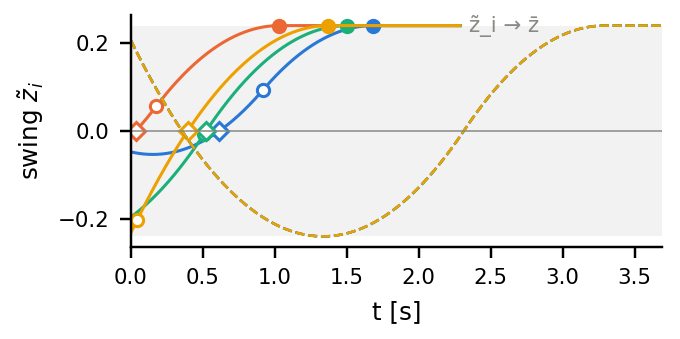
\includegraphics[width=\columnwidth]{profile_a_swings.png}\\[-2pt]
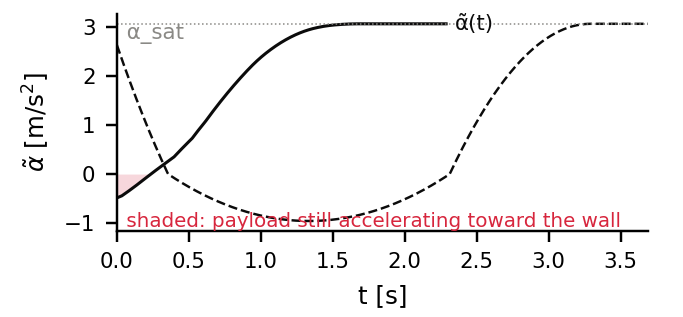
\includegraphics[width=\columnwidth]{profile_b_authority.png}\\[-2pt]
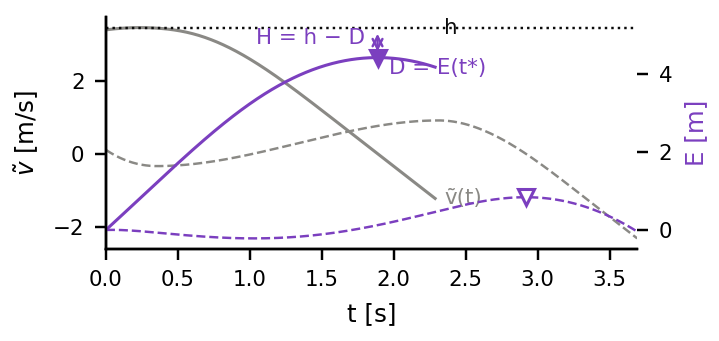
\includegraphics[width=\columnwidth]{profile_c_excursion.png}
\caption{A reserved swing (top) changes the cable directions and increases available braking (middle). The barrier subtracts the maximum wallward excursion $\max_t E(t)$ from the current distance $h$ (bottom). Solid and dashed curves are two example states.}\label{fig:profile}
\vspace{-5pt}
\end{figure}

\begin{lemma}[Envelope and monotonicity]\label{lem:envelope}
(i) Every $\zeta(\cdot)$ with absolutely continuous derivative, $\zeta(0)=\zeta$, $\dot\zeta(0)=\omega$, $|\ddot\zeta|\le\nu$ a.e., and $\zeta\le\bar\zeta$ satisfies $\zeta(t)\le\tilde\zeta(t;\zeta,\omega)$ for all $t\ge0$. (ii) $\tilde\zeta(t;\zeta,\omega)$ is nondecreasing in $\zeta$ and $\omega$ on $\mathcal{V}(\nu,\bar\zeta)$. (iii) $\Dres$ is nondecreasing in $v$, nonincreasing in every $\zeta_i$ and $\dot\zeta_i$, and locally Lipschitz; along the maneuver started at $x_0$, $\Dres(x(t))=\max_{s\ge t}\int_0^s\tilde v(\cdot;x_0)-\int_0^t\tilde v(\cdot;x_0)$.
\end{lemma}
\begin{proof}[Proof scheme]
Write $S(\zeta)=\sqrt{2\nu(\bar\zeta-\zeta)}$. A feasible trajectory moving toward $\bar\zeta$ must satisfy $\dot\zeta\le S(\zeta)$, or even full braking would overshoot. Before the switch $t_1$, $\tilde\zeta$ uses the largest acceleration $\nu$; afterwards it follows $\dot{\tilde\zeta}=S(\tilde\zeta)$ to $\bar\zeta$. A first crossing from below either contradicts maximal acceleration before $t_1$ or forces both motions to coincide on the stopping curve after $t_1$. This proves (i). Differentiation of the two polynomial branches in \eqref{eq:profile} gives nonnegative initial-state sensitivities on $\mathcal V$, proving (ii). Monotonicity of $\ua$ then orders $E(t)$ for every $t$, and maximization preserves that order. On compact initial-state sets the swing arrival times and the maximizing times are uniformly bounded because $\ua_{\rm sat}>0$; taking the maximum of the resulting locally Lipschitz family proves (iii). Restarting the swing at time $t$ reproduces its remaining trajectory, giving the stated time-shift identity.
\end{proof}

\subsection{Main result}\label{sec:main}

At regular swing states, for fixed $t$, $E(t;x)$ is continuously differentiable in $(v,\zeta,\dot\zeta)$, because \eqref{eq:profile} is continuously differentiable in its initial data (one-sided at $(\bar\zeta,0)$) and the integration over $s$ smooths the breakpoints of $\ua$, which each $\tilde\zeta_i$ meets only at isolated times except while held at $\bar\zeta$. At these regular states, Danskin's theorem \cite{clarke1990optimization} gives the directional derivative
\begin{equation}
\Dres'(x;\delta)=\max_{t\in T^\star(x)}\nabla_xE(t;x)\tr\delta
\label{eq:dirder}
\end{equation}
in directions $\delta$ along which the state stays in the domain of $\Dres$. At a degenerate swing state, use the upper right Dini derivative instead of the displayed gradient formula. For an admissible $u$, let $F_u(x)$ be the state derivative and define $H'(x;F_u(x))$ as this Dini derivative; at regular states it equals $-v-\Dres'(x;F_u(x))$, the ordinary derivative $\dot H(x,u)$ when the maximizing time is unique. On states with all $(\zeta_i,\dot\zeta_i)\in\mathcal{V}(\nu^{\mathrm{rel}},\bar\zeta)$, let $\Drel$ be \eqref{eq:D} computed with $(\oa,\nu^{\mathrm{rel}})$ in place of $(\ua,\nu)$, the stopping distance of an optimistic system that swings and brakes as hard as any admissible input allows, and let $\gamma$ be a locally Lipschitz extended class-$\mathcal{K}$ function.

\begin{theorem}[Inner and outer bounds]\label{thm:sandwich}
Let the system have second-order authority along $h$ on $\Xop$ with data $(\ua,\oa,\nu,\nu^{\mathrm{rel}},\bar\zeta)$, and let $\ua_{\mathrm{sat}}>0$. Then:
\begin{enumerate}
\item[(i)] $\Xrf$ is controlled invariant. For every $x\in\Xrf$, $K_H(x):=\{u\ \text{admissible}:\ H'(x;F_u(x))\ge-\gamma(H(x))\}$ contains $\plan(x)$. Every solution generated by a measurable selection $u(t)\in K_H(x(t))$ from $x(0)\in\Xrf$ that keeps $(\zeta_i,\dot\zeta_i)\in\mathcal{V}(\nu,\bar\zeta)$ satisfies $h(t)\ge H(x(t))\ge0$ for all $t\ge0$.
\item[(ii)] $\Viab(\mathcal{C})\subseteq\{x\in\Xop:\ (\zeta_i,\dot\zeta_i)\in\mathcal{V}(\nu^{\mathrm{rel}},\bar\zeta)\ \forall i,\ h\ge\Drel(x)\}$.
\item[(iii)] If $\ua\equiv\bar\alpha>0$, then $\Dres=\pos{v}^2/(2\bar\alpha)$ and $\Xrf$ is the classical safe set of a double integrator.
\end{enumerate}
\end{theorem}
\begin{proof}
(i) Under $\plan$ from $x_0\in\Xrf$, Lemma~\ref{lem:envelope}(iii) and $h(t)=h_0-\int_0^tv$ give $H(x(t))=h_0-\max_{s\ge t}\int_0^s v$, nondecreasing in $t$; $\plan$ keeps the state in $\Xop$ and the swing states in $\mathcal{V}$, so $\Xrf$ is forward invariant under $\plan$, hence controlled invariant. Next, the swing restarted at a later state of the maneuver is the remaining part of the swing started at $x$, so the derivative of $E(t;\cdot)$ along $F_{\plan}(x)$ equals $\tilde v(t;x)-v$ at regular states, and by \eqref{eq:dirder}, $H'(x;F_{\plan}(x))=-\max_{t\in T^\star(x)}\tilde v(t;x)$. Every maximizing time $t>0$ is a stationary point of $E(\cdot;x)$, so $\tilde v(t;x)=0$, and $t=0$ maximizes only if $v\le0$; hence $H'(x;F_{\plan}(x))\ge0\ge-\gamma(H(x))$ at regular states. The preceding time-shift identity gives the same inequality for the Dini derivative along $\plan$ at degenerate states. Finally, along a solution generated by $K_H$ that keeps the swing states in $\mathcal{V}$, $\Dres$ is locally Lipschitz \cite{clarke1990optimization}, so $H(x(t))$ is continuous with derivative $H'(x;\dot x)\ge-\gamma(H)$ a.e., and the comparison argument for nonsmooth barriers \cite{glotfelter2017nonsmooth} gives $H\ge0$; $h\ge H$ since $\Dres\ge0$.

(ii) Let $x_0\in\Viab(\mathcal{C})$ and let an admissible input keep the solution in $\mathcal{C}$. By (C2), $(\zeta_i,\dot\zeta_i)\in\mathcal{V}(\nu^{\mathrm{rel}},\bar\zeta)$ at all times, and by Lemma~\ref{lem:envelope}(i) with $\nu^{\mathrm{rel}}$, $\zeta_i(t)\le\tilde\zeta_i^{\mathrm{rel}}(t)$. By (C1) and the monotonicity of $\oa$, $b(t)\le\oa(\zeta(t))\le\oa(\tilde\zeta^{\mathrm{rel}}(t))=\tilde\alpha^{\mathrm{rel}}(t;x_0)$, so $v(t)\ge\tilde v^{\mathrm{rel}}(t;x_0)$ and $\min_th(t)\le h_0-\Drel(x_0)$; if $h_0<\Drel(x_0)$, the solution leaves $\mathcal{C}$.

(iii) $\tilde\alpha\equiv\bar\alpha$ gives $\tilde v=v-\bar\alpha t$ and $\max_t\int_0^t\tilde v=\pos{v}^2/(2\bar\alpha)$.
\end{proof}

Together, (i) and (ii) give $\Xrf\subseteq\Viab(\mathcal{C})\subseteq\{h\ge\Drel\}$, which answers problems (a) and (b) with $\mathcal{S}=\Xrf$; Sec.~\ref{sec:filter} answers (c). The gap $\Dres-\Drel$ is what the division of the input costs and vanishes in case (iii). Part (i) is a backup-CBF guarantee \cite{gurriet2020scalable,chen2021backup} with $\plan$ as the backup controller, but the closest approach along the backup trajectory has the closed form \eqref{eq:D} instead of being simulated, and the same data yield the outer bound (ii). The sets $\Xrf$ and $\Cho$ need not be nested.

\subsection{Application to the cable system}\label{sec:cable}

\begin{assumption}[Swing reserve]\label{ass:nu}
There exist $\nu,\nu_w>0$ and $\rho_i^{\mathrm{fb}}\ge0$ such that, for every $i$, $\sec\theta_q\sqrt{\bar\eta_{z,i}^2+\bar\eta_{w,i}^2}+\rho_i^{\mathrm{fb}}\le\rho_i$, where $\bar\eta_{z,i}:=m_i(l_i\nu+a_{\max}+l_i\bar\omega^2\bar z)$ and $\bar\eta_{w,i}:=m_i(l_i\nu_w+a_{\max}+l_i\bar\omega^2\bar w)$.
\end{assumption}

\begin{assumption}[Swing-rate consistency]\label{ass:op}
$\bar\omega^2\ge\sec^2\theta_q\,(4\nu\bar z+4\nu_w\bar w)$.
\end{assumption}

Assumption~\ref{ass:nu} reserves, within $\rho_i$, the perpendicular thrust needed to impose any $\ddot z_i\in[-\nu,\nu]$ and $\ddot w_i\in[-\nu_w,\nu_w]$ against the coupling terms of Lemma~\ref{lem:structure}(b), the factor $\sec\theta_q$ accounting for the non-orthogonality of the two swing directions on the sphere, and keeps $\rho_i^{\mathrm{fb}}$ for feedback; Assumption~\ref{ass:op} makes the swing-rate bound of \eqref{eq:Xop} hold on the admissible swing sets.

\begin{proposition}[The cable system has second-order authority]\label{prop:instance}
Let Assumptions~\ref{ass:split}, \ref{ass:nu}, and \ref{ass:op} hold, let $d_L=d_i=0$, and let $\zeta_i:=z_i$. Then \eqref{eq:load}--\eqref{eq:veh} has second-order authority along $h$ on $\Xop$ with $\ua=\alpha_y$ of \eqref{eq:authority},
\begin{align}
\oa(z)=\min\Big\{\tfrac{1}{m_L}\textstyle\sum_i&\phi^{\mathrm{rel}}_i(z_i),\label{eq:oa}\\
 &a_{\max}\sec\theta_q\,\max_i\pos{z_i}\Big\},\nonumber
\end{align}
where $\phi^{\mathrm{rel}}_i$ is $\phi_i$ with $\bar T_i^{\mathrm{rel}}:=f_{\max,i}+m_ia_{\max}+m_il_i\bar\omega^2$; $\nu$ of Assumption~\ref{ass:nu}; $\nu^{\mathrm{rel}}:=\max_i(\frac{f_{\max,i}}{m_il_i}+\frac{a_{\max}}{l_i}+\bar\omega^2)$; and $\bar\zeta=\bar z$. The map of (C3) sets $T_i=\bar T_i$ if $z_i>0$ and $T_i=T_{\min}$ otherwise, and steers each $w_i$ within $\mathcal{V}(\nu_w,\bar w)$.
\end{proposition}
\begin{proof}[Proof scheme]
For (C1), $T_i\le f_{\max,i}+m_i a_{\max}+m_il_i\bar\omega^2$ follows from Lemma~\ref{lem:structure}(a). The tension cone also gives $\sum_iT_i\cos\theta_q\le m_La_{\max}$, which bounds $b$ by the second term of \eqref{eq:oa}. Projecting Lemma~\ref{lem:structure}(b) onto $y$ establishes (C2). For (C3), choose the tensions that realize $\ua$ and prescribe $\ddot z_i\in[-\nu,\nu]$ plus a transverse $\ddot w_i\in[-\nu_w,\nu_w]$ that keeps $w_i$ in its stopping set. The Gram matrix of $(P_iy,P_ir)$ has eigenvalues $1$ and $1-z_i^2-w_i^2\ge\cos^2\theta_q$, so the required perpendicular thrust has norm at most $\sec\theta_q\sqrt{\bar\eta_{z,i}^2+\bar\eta_{w,i}^2}\le\rho_i$. Assumption~\ref{ass:split} then realizes the tensions and swings simultaneously. Finally, $\|\dot q_i\|^2\le\sec^2\theta_q(\dot z_i^2+\dot w_i^2)\le\bar\omega^2$ on the product of the swing stopping sets, proving that the trajectory stays in $\Xop$.
\end{proof}

The second term of \eqref{eq:oa} comes from the cone of \eqref{eq:U}: since $\sum_iT_i\cos\theta_q\le e_3\tr\sum_iT_iq_i\le m_La_{\max}$, one has $b=\frac{1}{m_L}\sum_iT_iz_i\le a_{\max}\sec\theta_q\max_i\pos{z_i}$. With all cables at $\bar z$, $\Drel=\pos{v}^2/(2a_{\max}\bar z\sec\theta_q)$ against $\Dres=\pos{v}^2/(2\ua_{\mathrm{sat}})$ with $\ua_{\mathrm{sat}}=\frac{1}{m_L}\sum_i\bar T_i\bar z$; where the cables must first swing, the gap is set by $\nu$ against $\nu^{\mathrm{rel}}$.

\begin{proposition}[Computation and decomposition]\label{prop:decomp}
For $t_j\in T^\star(x)$, the time derivative of $h-E(t_j;\cdot)$ under $u$ is
\begin{align}
\dot H_j(x,u)=-v&+t_j\,b\label{eq:Hdot}\\
&-\sum_{i}\big(\partial_{z_i}E(t_j;x)\,\dot z_i+\partial_{\dot z_i}E(t_j;x)\,\ddot z_i\big),\nonumber
\end{align}
with $b=\frac{1}{m_L}\sum_iT_iz_i$ and $\ddot z_i=\frac{1}{m_il_i}y\tr u_i^\perp-\frac{1}{l_i}y\tr P_ia-\|\dot q_i\|^2z_i$, and $H'(x;F_u(x))=\min_j\dot H_j(x,u)$ at regular states. Moreover: (a) $\Dres$, $T^\star$, and the coefficients of \eqref{eq:Hdot} depend on the state only through $(v,\{z_i,\dot z_i\}_i)$ and are computed exactly in $O(N\log N)$ arithmetic operations, because $E(\cdot;x)$ is piecewise quartic with at most $4N$ breakpoints; forming all gradient rows additionally takes $O(N|T^\star|)$ time; (b) given a common value $\hat a$ of the specific force, each constraint $\dot H_j\ge-\gamma(H)$ splits into $N$ affine constraints, one per quadrotor on $(T_i,u_i^\perp)$, whose right-hand sides sum to $-\gamma(H)+v$ once the consistency equation $m_L\hat a=\sum_iT_iq_i$ is also enforced; (c) without a common $\hat a$, the local constraints are neither necessary nor sufficient.
\end{proposition}
\begin{proof}[Proof scheme]
At a regular state, $\partial_vE(t;x)=t$ and the chain rule gives \eqref{eq:Hdot}; Danskin's formula makes the derivative of $H=h-\max_tE(t)$ the minimum over its active times. Every $\tilde z_i$ is piecewise quadratic, with at most its switch, arrival, and two zero crossings as breakpoints. Thus $\tilde\alpha$ is piecewise quadratic, $E$ piecewise quartic, and candidate maximizers are interval endpoints or roots of cubic $\tilde v$. Sorting $O(N)$ events takes $O(N\log N)$ arithmetic operations; all active gradient rows additionally take $O(N|T^\star|)$. For a committed common $\hat a$, \eqref{eq:Hdot} is a sum of local affine terms, but validity also requires $m_L\hat a=\sum_iT_iq_i$; otherwise the local rows need not represent the actual coupled plant.
\end{proof}

\begin{remark}[Scope of the guarantee]\label{rem:inner}
The certificate assumes an exact taut-cable model, continuously updated thrust commands, and a feasible transverse swing reserve. Wind, mass errors, actuator tracking, slack cables, and zero-order-hold inputs require additional error bounds and are \emph{not} covered by Theorem~\ref{thm:sandwich}. In particular, continuity and local Lipschitzness of $\Dres$ do not by themselves give a numerical sampled-data margin.
\end{remark}



\section{Safety Filter}\label{sec:filter}

The decision variables are the tensions $T\in\R^N$ and the perpendicular components $u^\perp=(u_1^\perp,\dots,u_N^\perp)$, $u_i^\perp\perp q_i$; the thrust vector of quadrotor $i$ is $s_i(T)q_i+u_i^\perp$ with $a=\frac{1}{m_L}\sum_jT_jq_j$ in Lemma~\ref{lem:structure}(a). For each swing coordinate $\zeta\in\{z_i,w_i\}$ with data $(\nu_\zeta,\bar\zeta_\zeta)\in\{(\nu,\bar z),(\nu_w,\bar w)\}$, let $\partial^\pm_\zeta$ be the upper and lower boundaries of $\mathcal{V}(\nu_\zeta,\bar\zeta_\zeta)$. Given the nominal thrust vectors $u_i^{\mathrm{nom}}$, the filter solves
\begin{subequations}\label{eq:filter}
\begin{align}
&\min_{T,u^\perp}\ \textstyle\sum_i\|s_i(T)q_i+u_i^\perp-u_i^{\mathrm{nom}}\|^2 \\
&\text{s.t.}\  u\in\mathcal{U}(x), \label{eq:filter-thrust}\\
& \dot H_j(x,T,u^\perp)\ge-\gamma(H(x))\quad \forall\,t_j\in T^\star(x), \label{eq:filter-H}\\
& \ddot\zeta\le-\nu_\zeta\mathbf{1}[\dot\zeta>0]\ \text{on}\ \partial^+_\zeta,\ \ \ddot\zeta\ge\nu_\zeta\mathbf{1}[\dot\zeta<0]\ \text{on}\ \partial^-_\zeta, \label{eq:filter-box}
\end{align}
\end{subequations}
for every $i$ and every swing coordinate. Constraint \eqref{eq:filter-H} is the barrier condition of Thm.~\ref{thm:sandwich}(i) written with Prop.~\ref{prop:decomp}, one affine constraint per maximizing time, and \eqref{eq:filter-box} are the tangency conditions that are necessary for the swing states to remain in their admissible sets \cite{aubin1991viability}; a class-$\mathcal{K}$ condition on a function that vanishes on $\partial\mathcal{V}$ would forbid the time-optimal swing, which reaches that boundary in finite time. At regular states the program is a second-order cone program with $3N$ variables, with global coupling through the common payload force $a$, the thrust reconstructions $s_i(T)$, and the cone in \eqref{eq:U}. An affine split of the barrier rows still requires enforcing the common-force consistency equation. At degenerate swing states, the displayed gradient rows are not asserted to characterize the Dini condition; the filter applies the known feasible backup input $\plan$ instead.

By Thm.~\ref{thm:sandwich}(i), the filter is feasible at regular states of $\Xrf$ and applies $\plan$ at degenerate states; at regular states $\plan(x)$ satisfies \eqref{eq:filter-H} with slack at least $\gamma(H)$; along every solution whose swing states remain admissible, $h\ge H\ge0$.

In a distributed implementation, the broadcast $\hat a$ must equal the specific force generated by the simultaneous tension commands, and the cone and thrust constraints still require coordination. A lagged broadcast is not a feasibility certificate.

Uncertain mass requires checking the coupled thrust, tension, and swing reserve for every allowed mass; replacing $m_L$ only in the authority formula is insufficient for a robust guarantee.



% The figures of this section are declared ahead of its text, in the order of their numbers.
\begin{figure*}
\centering
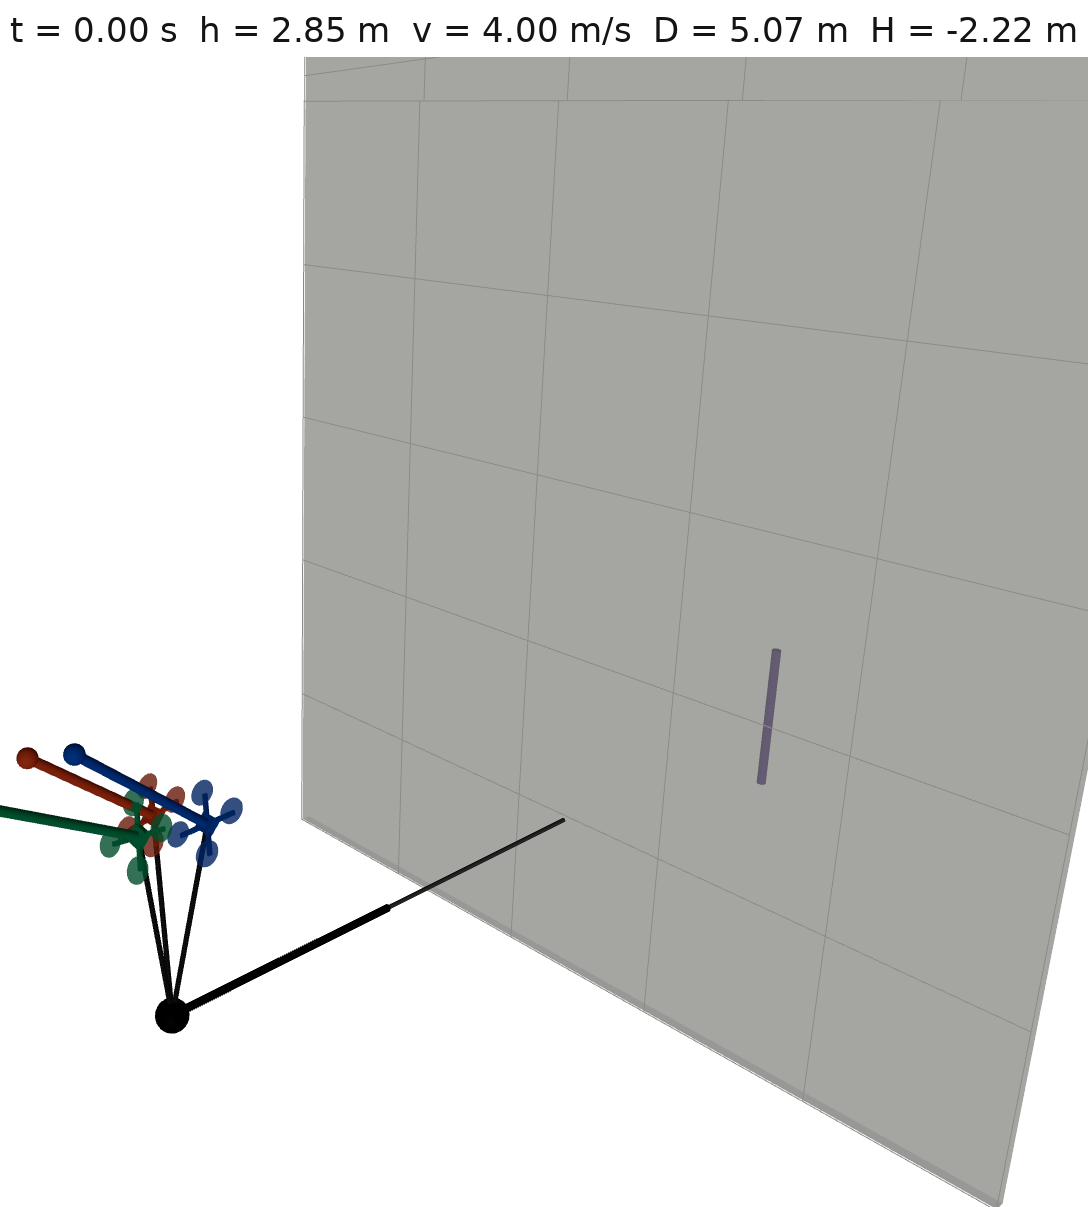
\includegraphics[width=0.24\textwidth]{sequence_0.png}\hfill
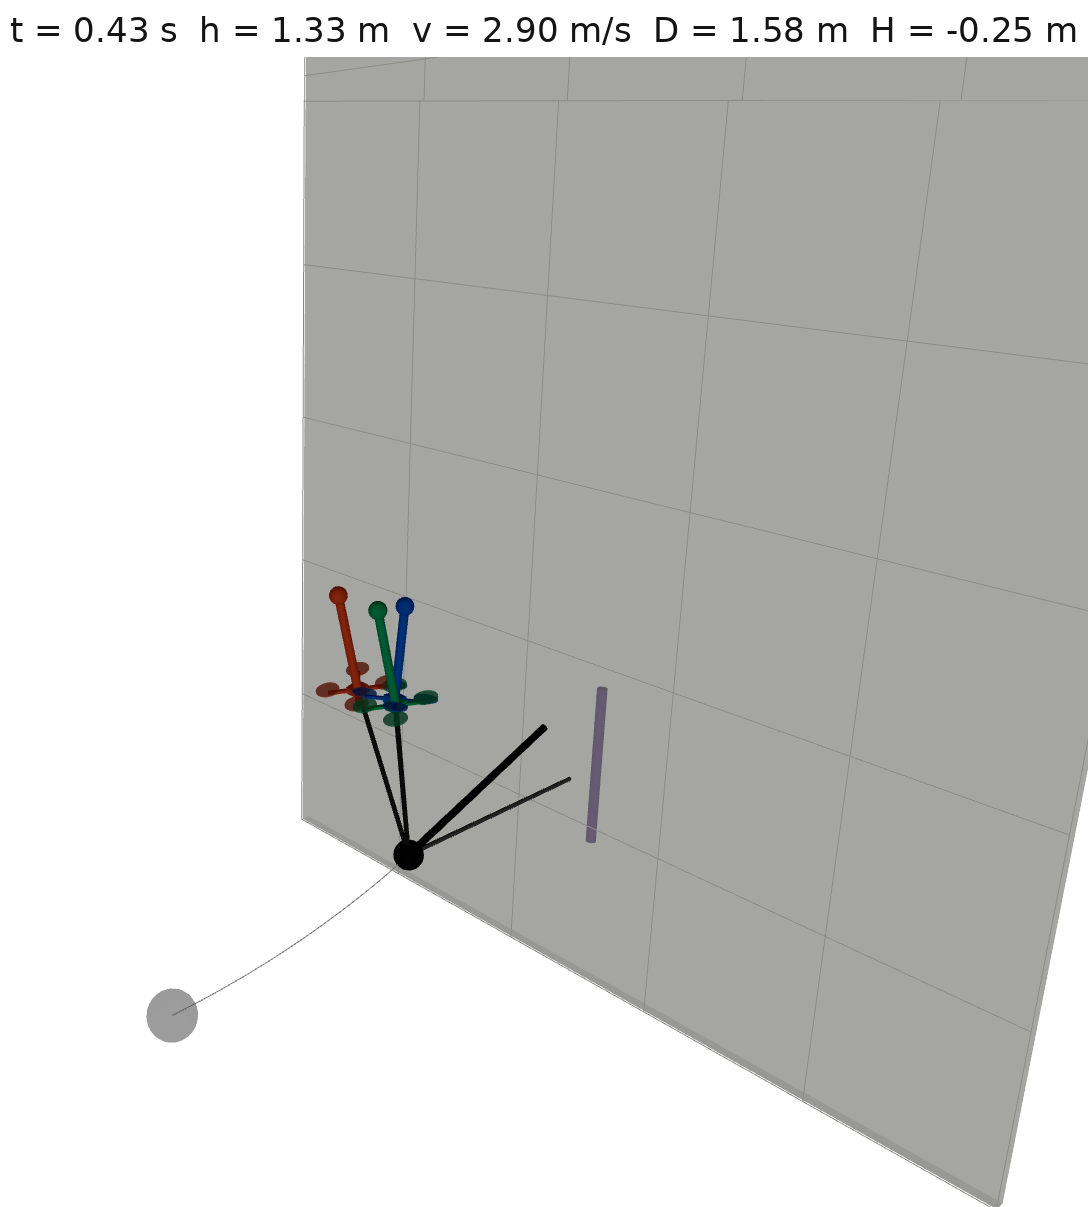
\includegraphics[width=0.24\textwidth]{sequence_1.png}\hfill
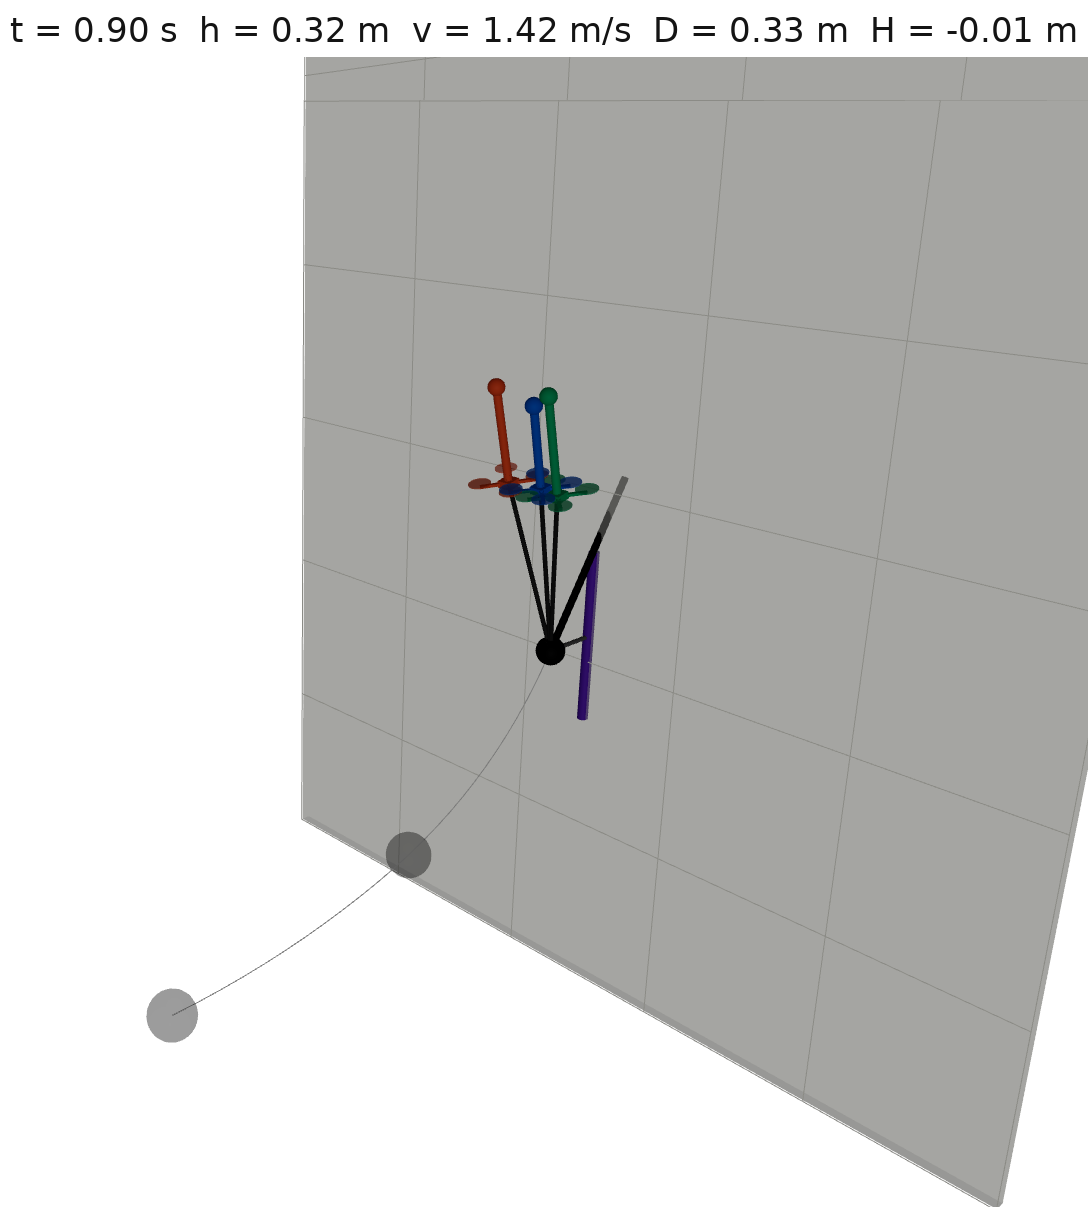
\includegraphics[width=0.24\textwidth]{sequence_2.png}\hfill
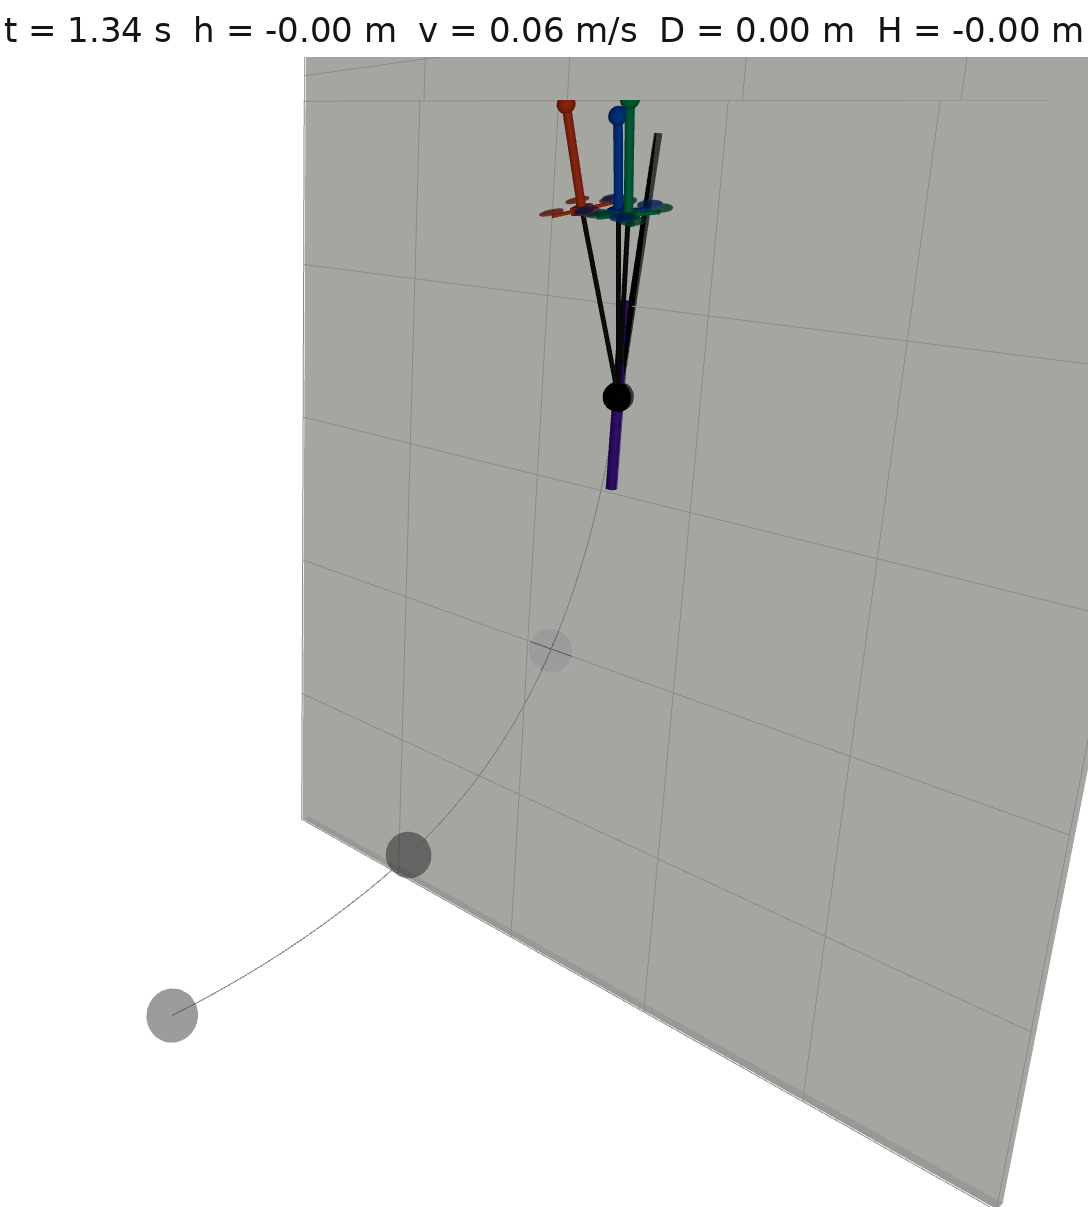
\includegraphics[width=0.24\textwidth]{sequence_3.png}
\caption{Four frames of a collocation trajectory for the mixed cable configuration (B) at $v_0=4\,\mathrm{m/s}$ from $h_0=0.56\Dres$. The quadrotors reposition their cables behind the payload and enter $\Xrf$. The frames show one example of a safe trajectory; the kernel was not computed exhaustively.}\label{fig:sequence}
\vspace{-5pt}
\end{figure*}

\begin{figure}[t]
\centering
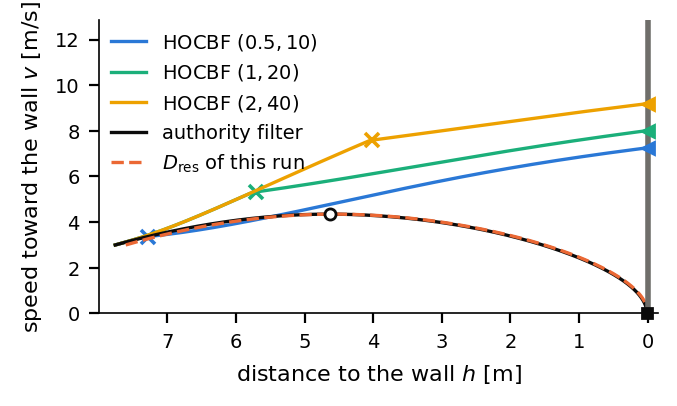
\includegraphics[width=0.95\columnwidth]{exact_comparison.png}
\caption{Exact taut-cable model, one initial state of the certified set $\mathcal S$ and one adversarial nominal input, in the plane of wall distance and approach speed; the wall is the right edge. The HOCBF filters lose feasibility (crosses) while every cable leans toward the wall, and reach the wall (triangles). The authority filter brings every cable into the braking half-space (circle) and stops at the wall (square); the dashed curve shows $\Dres$ of its states.}\label{fig:exact}
\end{figure}

\begin{figure}[t]
\centering
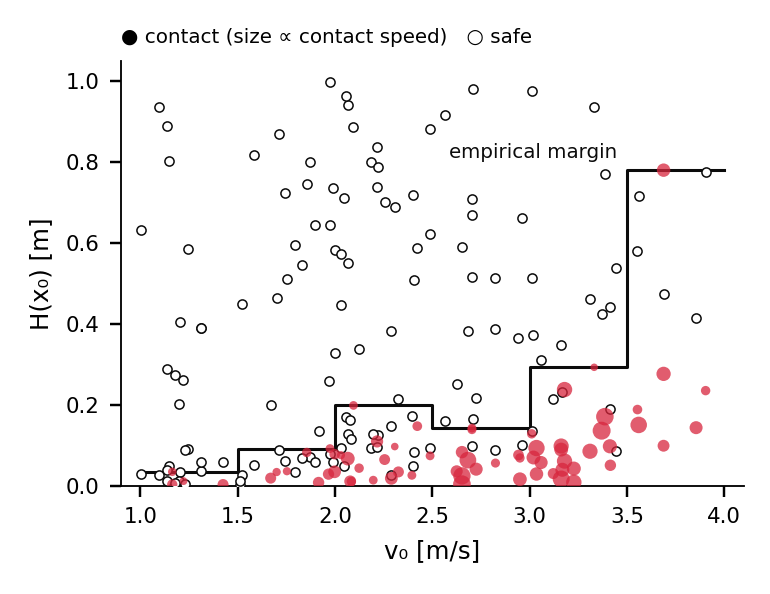
\includegraphics[width=0.82\columnwidth]{sampled_margin_map.png}
\caption{Sampled-filter runs in the $(v_0,H(x_0))$ plane (filled: wall contact; open: no contact). The step gives the largest observed contact margin in each speed bin. The observed threshold is not a certified sampled-data bound.}\label{fig:sampled}
\end{figure}

\begin{figure}[t]
\centering
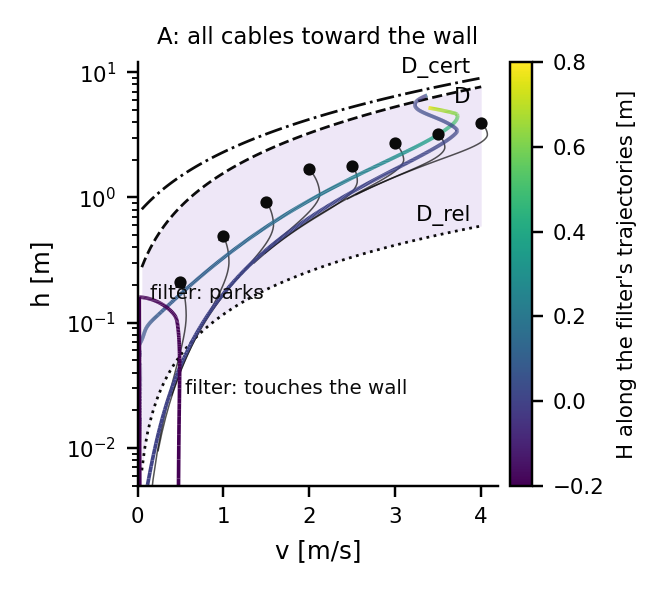
\includegraphics[width=0.90\columnwidth]{sandwich_a.png}
\caption{Viability band for configuration A, cables initially leaning toward the wall: reserved (dashed) and optimistic (dotted) stopping distances. Dots are the smallest \emph{found and re-simulated} collocation trajectories; they do not prove where the kernel boundary lies. Colored curves are two closed-loop trajectories of the sampled authority filter.}\label{fig:sandwich-a}
\vspace{-5pt}
\end{figure}

\section{Numerical study}\label{sec:sim}
Figure~\ref{fig:profile} illustrates the predicted swing profiles. The team has four $1.5\,\mathrm{kg}$ quadrotors carrying a $1\,\mathrm{kg}$ point payload on $1\,\mathrm m$ cables, with $T_{\min}=1\,\mathrm N$, $f_{\max}=44\,\mathrm N$, $\bar T_i=3.2\,\mathrm N$, $\rho_i=34\,\mathrm N$, $a_{\max}=13\,\mathrm{m/s^2}$, $\theta_q=20^\circ$, $\bar z=0.239$, $\bar w=0.171$, $\bar\omega=1\,\mathrm{s^{-1}}$, and $\nu=\nu_w=0.5\,\mathrm{s^{-2}}$. The thrust-reserve bound holds: $\sqrt{(\bar T_i+m_ia_{\max}+m_il_i\bar\omega^2)^2+\rho_i^2}=41.73\,\mathrm N<f_{\max}$. The code and trial videos are available online.\footnote{\url{https://github.com/Hadi-Hajieghrary/Authority_Barriers}}

\textcolor{red}{\textbf{SUGGESTION:} Add a compact experiment-configuration table specifying the $\gamma$ functions and gains, initial-state sampling procedure and seeds, integration settings, solver tolerances, and code version.  Report computation times for the complete filter in Equation~(17), including its altitude constraints.  Specify the numerical backup-CBF baseline's integration horizon and sensitivity-calculation method.  Use comparable accuracy and common hardware for the timing comparison.  State the software environment and number of evaluations.  Report typical and maximum observed computation times and compare them with the stated controller update periods.}

\textcolor{red}{\textbf{WHY:} These settings are needed to reproduce the reported feasibility and wall-contact results.  The comparison of $129$~s against $6$~ms requires enough implementation detail to distinguish an analytical advantage from differences in numerical accuracy or baseline implementation.  The existing wall-only timing measurements do not establish the computational cost of the complete certified filter.  Reporting timing variability also helps reviewers assess whether the implementation can support the proposed update periods.}

\emph{Exact model.} Theorem~\ref{thm:sandwich}(i) was tested in its own setting: the authority filter \eqref{eq:filter} on the taut-cable model under a zero-order hold, with $T^{\mathrm h}_i=2.7\,\mathrm N$, $\nu'=0.4\,\mathrm{s^{-2}}$, $c_\downarrow=5$ and $c_\uparrow=2\,\mathrm{m/s^2}$, $\epsilon=0.1\,\mathrm s$, $c_a=1.25$, and the band $0\le\chi\le45\,\mathrm m$. The 100 initial states have random swing states, speeds of $1$--$4\,\mathrm{m/s}$, and $H(x_0)\in[0,0.05\,\Dres(x_0)]$, between $1\,\mathrm{mm}$ and $0.38\,\mathrm m$; the nominal input is adversarial: the full thrust of every quadrotor toward the wall, tilted $40^\circ$ upward; a trial lasts $6\,\mathrm s$. Table~\ref{tab:exact} gives the result. With a period of $1\,\mathrm{ms}$ the barrier stayed above $-0.05\,\mathrm{mm}$, one trial reached the wall, by $2\,\mu\mathrm m$, and the altitude stayed in its band in every trial; the payload climbed by up to $29.9\,\mathrm m$. 

\textcolor{red}{SUGGESTION: Strengthen the numerical verification of the complete filter in Equation~(17), including its altitude and swing constraints.  Repeat identical initial states and nominal inputs with command holds of $1$, $0.5$, and $0.25$~ms.  At each fixed hold, independently refine the integration settings and solver tolerances.  Report minimum wall clearance, minimum barrier values, and any input or operational-constraint violations.  Evaluate these quantities between controller updates.  Determine how the reported $2,\mu\mathrm{m}$ wall penetration changes under refinement.  Clearly distinguish the continuous-time guarantee from its sampled implementation.}

\textcolor{red}{WHY: Theorem~9(i) provides a continuous-time guarantee, while Table~I evaluates commands applied through a zero-order hold.  The small wall penetration could reflect sampling, integration error, or optimization tolerances.  Independent refinement is needed to distinguish these effects.  The full-order wall-only trials omit constraints from the certified filter and introduce slack-cable dynamics.  Those trials demonstrate limitations but cannot verify the complete certificate under its stated assumptions.}

Figure~\ref{fig:exact} compares the authority filter with HOCBF filters with linear gains $(k_1,k_2)\in\{(0.5,10),(1,20),(2,40)\}\,\mathrm{s^{-1}}$ from one state with $v=3\,\mathrm{m/s}$, every cable at $z_i=-0.8\bar z$, and $h=1.02\,\Dres=7.76\,\mathrm m$. Each HOCBF program is feasible at the start and infeasible after $0.15$, $0.52$, and $0.78\,\mathrm s$, with every cable leaning toward the wall; its relaxation with a penalized slack reaches the wall at $7.3$--$9.2\,\mathrm{m/s}$. The authority filter has every cable in the braking half-space after $0.81\,\mathrm s$ and stops the payload $10\,\mathrm{mm}$ from the wall, with $H$ between $0.15$ and $0.01\,\mathrm m$. Without the bound on the swing accelerations, the filter follows the nominal input with swing accelerations of about $20\,\mathrm{s^{-2}}$, forty times $\nu$; the stopping distance then changes within one period by more than its gradient predicts, and the contacts multiply; a margin of the kind derived for sampled-data CBFs~\cite{breeden2022sampled} is not available for $\Dres$. With the hover floor the stopping distance from $3\,\mathrm{m/s}$ with every cable at $-\bar z$ is $9.18\,\mathrm m$, against $6.56\,\mathrm m$ with the floor $T_{\min}$ and the time-optimal swing: carrying the weight costs $2.6\,\mathrm m$.

\begin{table}[t]
\caption{The authority filter on the exact taut-cable model, 100 trials per row.}\label{tab:exact}
\centering\footnotesize\setlength{\tabcolsep}{4pt}
\begin{tabular}{@{}cccccc@{}}
\toprule
Period & $|\ddot\zeta|\le c_a\nu_\zeta$ & Contacts & Deepest & $\min H$ & $\chi$ in band\\
\midrule
$1\,\mathrm{ms}$ & yes & 1 & $0.002\,\mathrm{mm}$ & $-0.05\,\mathrm{mm}$ & 100\\
$5\,\mathrm{ms}$ & yes & 4 & $0.4\,\mathrm{mm}$ & $-7\,\mathrm{mm}$ & 100\\
$1\,\mathrm{ms}$ & no & 6 & $0.1\,\mathrm{mm}$ & $-13\,\mathrm{mm}$ & 97\\
$5\,\mathrm{ms}$ & no & 33 & $1.7\,\mathrm{mm}$ & $-104\,\mathrm{mm}$ & 100\\
\bottomrule
\end{tabular}
\end{table}

\emph{Full-order model.} The remaining trials use rigid quadrotors, spring--damper cables that can go slack, and a filter at $200\,\mathrm{Hz}$. They were run with the wall barrier alone, that is, with the floor $T_{\min}$ in $\phi_i$, the time-optimal swing, and neither \eqref{eq:filter-alt} nor the bound on the swing accelerations; the altitude is free in them, and the payload climbs by $54\,\mathrm m$ in one trial before it stops. All 690 HOCBF trials lost QP feasibility before a cable entered the braking half-space: the three gain pairs of Fig.~\ref{fig:exact}, each from 100 states with every cable leaning toward the wall at $2$--$4\,\mathrm{m/s}$, with thrust vectors applied directly and with a $1\,\mathrm{kHz}$ attitude loop, and from 30 states with three quadrotors. This does not establish initial feasibility for arbitrary gains. Of 100 trials started with $H(x_0)\in[0,0.05\,\Dres]$ under the adversarial nominal input, the sampled authority filter reached the wall in 59 despite a feasible QP at its sampling instants (Fig.~\ref{fig:sampled}); in 56 trials a cable was slack at some sample. The largest barrier loss was $0.85\,\mathrm m$ within one $5\,\mathrm{ms}$ hold; no contact was observed above an initial margin of $0.78\,\mathrm m$ in a second sweep of 100 states. This margin is empirical and holds for the tested distribution only. The attitude loop incurred $17$--$43\,\mathrm N$ tracking errors during command jumps.

\textcolor{red}{\textbf{SUGGESTION:} Repeat the collocation comparison using the same taut-cable dynamics, vehicle count, input limits, operational constraints, and altitude band as the certified filter.  Match all initial-state components except the wall clearance being minimized.  Specify the tension floors and swing maneuver used to compute $D$ in each comparison.  Verify the hover, thrust, and swing reserve assumptions for each vehicle configuration.  Re-simulate candidate trajectories and check every constraint.  Report the smallest found safe clearance relative to $D$.  Include a representative tighter altitude band to assess practical usefulness.}

\textcolor{red}{\textbf{WHY:} The reported clearances of $0.25D$ to $0.55D$ come from searches with different model and constraint settings from the complete certificate.  Relaxed constraints can permit shorter stopping distances.  A matched comparison is needed to determine how much of the gap comes from the certificate's conservative construction.  Testing a tighter altitude band would also clarify its operating usefulness, given the reported climb of up to $29.9$~m.}

\emph{Conservatism.} Direct-collocation searches with three quadrotors covered three initial cable configurations at rest (A: $z_i=-0.15$; B: $z=(-0.15,0,0.15)$; C: $z_i=\bar z$) at eight speeds from $0.5$ to $4\,\mathrm{m/s}$, with each candidate subsequently simulated; like the full-order trials, they constrain the wall distance only. When cables already lean away from the wall, the observed feasible distance is about $0.97$--$0.98$ times $\Dres$; when a swing is required, feasible trajectories can begin at only $0.25$--$0.55\,\Dres$ (Fig.~\ref{fig:sandwich-a} shows configuration A). Figure~\ref{fig:sequence} shows one such trajectory. The large gap is driven in part by the reserved swing acceleration: $\nu=0.5\,\mathrm{s^{-2}}$ needs $1.96\,\mathrm{s}$ to cross the allowed angle range, while the physical thrust can reach the swing-rate limit much sooner, and Assumption~\ref{ass:op} admits no $\nu$ above $0.54\,\mathrm{s^{-2}}$ at this rate limit. A collocation success gives an example trajectory, but a failure does not locate the viability boundary, so the evidence supports the qualitative gap between the two models and validates neither set inclusion.

\emph{Cost.} A backup filter that integrates $\plan$ numerically \cite{chen2021backup} reproduced $\Dres$ within a relative error of $1.1\cdot10^{-6}$ and the commands of the filter within $0.4\,\%$ of $f_{\max}$ at 60 states, at $129\,\mathrm s$ per evaluation against $6\,\mathrm{ms}$. In Python with the solver Clarabel, evaluating $\Dres$ takes $0.5$--$0.6\,\mathrm{ms}$ and the filter with the wall barrier $2$--$4.5\,\mathrm{ms}$ for two to eight quadrotors, close to the $5\,\mathrm{ms}$ sampling period; solver failures, model mismatch, and inter-sample excursions preclude a real-time guarantee.


\section{Conclusion}\label{sec:conclusion}
Cable geometry makes braking authority a controlled state: the team brakes only as hard as the cable directions allow, and these change at a bounded rate. An initially feasible HOCBF can lose feasibility when the geometry cannot change quickly enough, under the stated gain-dependent condition. A support-function calculation and an explicit swing-and-brake maneuver give useful continuous-time inner and outer viability bounds, and the argument extends to every system with second-order authority. The inner bound is conservative where the cables must first swing: safe trajectories were found from as little as $0.25\,\Dres$ there, against $0.97$--$0.98\,\Dres$ with the cables already behind the payload; the reserved swing acceleration accounts for part of this gap.

The simulations also reveal that the current sampled filter and physical cable model do not satisfy the theorem's hypotheses: the barrier lost up to $0.85\,\mathrm m$ within one $5\,\mathrm{ms}$ hold; of 100 trials started near the boundary of the safe set, 56 had a slack cable and 59 reached the wall. A certified sampled-data bound, coordinated force allocation, and reproducible full-order validation are the next requirements for a deployment claim.



\bibliographystyle{IEEEtran}
\bibliography{References}

\end{document}
